
\chapter{General Conclusions}\label{chapter6}

Formation and evolution of velocity multistreams in the dark matter Universe plays a vital role in the formation of large scale structures in the Universe. In this thesis, we have analyzed this multi-stream field in cosmological context -- from dark matter halo environments to connectivities in the single streaming voids. It has been demonstrated that the studies of the Lagrangian sub-manifold not only provide a novel way of looking at the cosmos, but also boost our current knowledge of the dark matter Universe. 

This final chapter encapsulates significant findings of our work. In addition, we also highlight a few interesting avenues for future research using the Lagrangian sub-manifold.      

\section{Summary of major results}

The full dynamical state of cold dark matter can be described as a three-dimensional sub-manifold
in six-dimensional phase space - the dark matter sheet. In our study we use a Lagrangian sub-manifold ${\bf x} = {\bf x}({\bf q},t)$ 
(where {\bf x} and {\bf q} are co-moving Eulerian and Lagrangian coordinates respectively), which 
is dynamically  equivalent to the dark matter sheet but is more convenient for numerical analysis. Projecting the Lagrangian sub-manifold at each point in the configuration space defines the multistream field  $n_{str}(\mathbf{x}, z)$. This integer-valued field is equivalent to counting the number of foldings in the sub-manifold and we numerically calculate by a Lagrangian tessellation scheme. The resulting multistream field is dynamical, positively correlated with matter density, and supplements our knowledge of spatial clustering. Our major results can be summarized as follows:

\begin{itemize}
% \subsection{Hierarchical structure of the dark matter web}
\item {\bf Hierarchical structure of the dark matter web: } The first study of the multi-stream environment of dark matter haloes in cosmological N-body simulations in the $\Lambda$CDM cosmology reported in Chapter \ref{chapter3} (first shown in \cite{Ramachandra2015}) shows that at the resolution of the simulation i.e. without additional smoothing, the cosmic web represents a hierarchical structure: each halo is embedded in the filamentary framework of the web predominantly  at the filament crossings, and each filament is embedded in the wall like fabric of the web at the wall crossings. 

Voids are uniquely defined by the local condition requiring to be a single-stream flow region. Within the dark matter web (regions with $n_{str} > 1$), the walls are regions where $n_{str} \cong 3$. The number of streams in the neighboring filaments is higher than in the neighboring walls. Finally, each halo or sub-halo is a local peak in the $n_{str}$ field. We demonstrated in Chapter \ref{chapter3} that the shells of streams around haloes are quite thin and the closest void region is typically within one and a half FOF radius from the center of the halo.

% number of streams is equal to three or a few.
% \subsection{Multistream view of the dark matter haloes}

\item {\bf Multistream view of the dark matter haloes: } In our simulation reported in Chapter \ref{chapter3}, simple virial density criterion corresponds to a global threshold of $n_{str} \geq 90$ for DM haloes. This shows a reasonably good correspondence with structure finders. A more sophisticated halo finding formulation is done in Chapter \ref{chapter5} assuming that the virialized haloes have convex boundaries. Closed and convex regions of the multistream field are hence isolated by imposing a positivity condition on all three eigenvalues of the Hessian estimated on the smoothed multistream field. In a single-scale analysis of high multistream field resolution and low softening length, the halo substructures with local multistream maxima are isolated as individual halo sites. This halo finding technique is free of any heuristic parameters, and may be extended to delineate filaments, walls, voids, as well as halo sub-structures. Agreement of halo summary statistics (like the halo mass function) of the multistream haloes with traditional halo finders (Friends-of-Friends and Spherical Over-density based techniques) is shown \cite{Ramachandra2017b}. As opposed to several other halo finders, this geometrical approach accounts for non-spherical boundaries, does not find any halo candidates in voids, and minimizes the need for post-processing in the production of halo catalogs for dark matter simulations.   

% \subsection{Topological transitions in the cosmic web}

\item {\bf Topological transitions in the cosmic web: } Topological connections in the single-streaming voids and multistreaming filaments and walls reveal a cosmic web structure different from traditional mass density fields, as shown in Chapter \ref{chapter4}. Single streaming voids occupy over 90 per cent of the dark matter Universe. A single void structure not only percolates the multistream field in all the directions, but also spans over 99 per cent of all the single-streaming regions. Sub-grid analyses on scales smaller than simulation resolution reveal tiny pockets of voids that are isolated by membranes of the structure. 

Rapid topological transitions are seen in matter density fields as well as multistream fields, i.e., at a given threshold (matter density or multistream), the filling fraction of the largest structure in the Universe dominates the excursion volume fraction. For the multistreaming excursion sets, the percolating structure is significantly thinner than the filaments in over-density excursion approach. We also demonstrated that the matter density field is more fragmented than the multistream field. 
 
\end{itemize}


\section{Future directions}

Although the scope of this thesis has primarily been multistream field and its application to cosmic structure formation, it is necessary to highlight other important physical insights derived from the Lagrangian sub-manifold. For instance, tracing the Lagrangian sub-manifold also provides rich insights into halo collapse modeling \cite{Neyrinck2016}. Recently, there have been attempts to improve N-body simulations (see \cite{Hahn2013}, \cite{Angulo2013a}, \cite{Angulo2013b}, \cite{Sousbie2015} and \cite{Hahn2016a}) by solving the Vlasav-Poisson equation using tessellations in the Lagrangian sub-manifold. Galaxy evolution and star formation in the context of multi streaming phenomenon are studied by \cite{Aragon-Calvo2016}. Problems of halo-core tracking, dynamical analysis of halo merger histories, halo and sub-halo disruption events and mass accretion of filaments and haloes may be revisited using Lagrangian sub-manifold.

This section reviews two of the potential avenues for interesting application of Lagrangian sub-manifold. One may track the {\it Flip-Flop} field -- to understand the rich and complex substructures within haloes. On the other hand, Lagrangian sub-manifold may also be used to identify caustic surfaces -- measure-zero surfaces in the DM Universe that have formally infinite density. 


\subsection{Flip-Flop analyses in Lagrangian field}

The integer value of Flip-flop in Lagrangian field, $n_{ff}(\mathbf{q})$ is increased by every swap of the Eulerian coordinates of the two neighboring DM particles. This number field is estimated in three dimensions by computing the Jacobian  $J(\mathbf{q}, t) = |\frac{\partial\mathbf{x}}{\partial\mathbf{q}}|$  on each particle at each time step. If the sign of the Jacobian changes, the number of flip-flops for the corresponding particles is increased by one. Details of calculation of flip-flop field and its significance in dynamical history of substructure formation is explained in \citep{Shandarin2016}, and summarized in Section \ref{sec:ZA}. This Lagrangian field $n_{ff}(\mathbf{q})$ for a cosmological simulation with $128^3$ DM particles and side length of $100 h^{-1} Mpc$ is shown in the left panel of \autoref{fig:ffq}. Halo environment analysis similar to one in Chapter \ref{chapter5} may allow us to identify and track the formation of DM haloes directly from the Lagrangian space. Alternatively, this also enables back-tracking the DM particles in halos cores and substructures all the way to the initial configurations in the simulation.  

\begin{figure}
\begin{minipage}[t]{.99\linewidth}
 \centering\includegraphics[width=5.7cm]{Chapter2/Plots/ffq.pdf} 
\centering\includegraphics[width=5.cm]{Chapter2/Plots/ff0_slice.pdf} 
 \centering\includegraphics[width=5.cm]{Chapter2/Plots/ff1_slice.pdf} 
\end{minipage}\hfill
\caption{Left panel: Lagrangian slice of the Flip-Flop field $n_{ff}(\mathbf{q})$ in a cosmological simulation with $L = 100 h^{-1} Mpc$. The values of $n_{ff}$ varies from $0$ to $15$. Center panel: Eulerian picture, only the particles with $n_{ff}(\mathbf{q}) = 0$. are shown. Red regions show regions with $n_{str}(\mathbf{x}) > 1$. Right panel: Eulerian picture, only the particles with $n_{ff}(\mathbf{q}) > 0$. are shown. Red regions show regions with $n_{str}(\mathbf{x}) > 1$.}
\label{fig:ffq}
\end{figure}


\begin{figure}
\begin{minipage}[t]{.99\linewidth}
%  \centering\includegraphics[width=5.cm]{Chapter2/Plots/PercPlot_ns.pdf} 
 \centering\includegraphics[width=8.cm]{Chapter2/Plots/PercPlot_ff.pdf} 
  \centering\includegraphics[width=8.cm]{Chapter2/Plots/PercPlot_ff_ns.pdf}  
\end{minipage}\hfill
\caption{Left panel: Percolation transition for the Flip-Flop, $n_{ff}(\mathbf{q})$. Shows the excursion set fraction $f_{ES}$ and the filling fraction $f_1$ for various flip-flop thresholds. Right panel: Percolation transition for the Flip-Flop field, $n_{ff}(\mathbf{q})$ and multi-stream field $n_{str}(\mathbf{x})$.}
\label{fig:percplot}
\end{figure}



Since the $n_{ff}$ field is defined on particles, mapping the field to Eulerian field is straightforward. Correspondence between the multistream field defined in Eulerian space $n_{str}(\mathbf{x})$ is shown in the middle and right panels of \autoref{fig:ffq}. Most particles that have not undergone a flip-flop are in the single-streaming region. In the multistreaming region, however, consists of particles with $n_{ff} = 0$ and $n_{ff} > 0$. On the other hand, $n_{ff} > 0$ particles are not found in single-streaming voids. 

Percolation analysis (similar to the multistream analysis in Chapter \ref{chapter4}) may also be done using the Flip-Flop in the Lagrangian field. \autoref{fig:percplot} shows topological transitions similar to ones in multistream and matter density fields shown in \autoref{fig:PercTh} and \autoref{fig:HaloFil}, except here we explore the connectivities in the Lagrangian space. This could reveal topological connections in the initial positions, and reveal whether or not the connections remain intact throughout the evolution of nonlinear gravitational collapse. 

% \begin{figure}
% \begin{minipage}[t]{.99\linewidth}
%  \centering\includegraphics[width=8.cm]{Chapter2/Plots/PercPlot_ff_ns.pdf}  
% \end{minipage}\hfill
% \caption{Percolation transition for the Flip-Flop, $n_{ff}(\mathbf{q})$ and multi-stream field $n_{str}(\mathbf{x})$.}
% \label{fig:perctransition}
% \end{figure}




\subsection{Caustics formation}



Existence of singularities is a distinguishing feature of collisionless DM collapse from that of baryonic matter. Caustic formation in the context of the ZA \citep{Zeldovich1970} was discussed earlier in Section \ref{sec:ZA} (also see \cite{Shandarin1989} for a detailed study of cosmic singularities). Theoretical characterization of caustic surfaces in a two dimensional gravitational collapse was studied by \citep{Arnold1982}. However, such analytical treatment is complicated in the three-dimensional case (See for example, the discussions in \citealt{Hidding2014}, \citealt{Feldbrugge2018}). Numerically, one may find the particles belonging to caustic surfaces by following the determinants of the volume elements in the Lagrangian sub-manifold. This result of such scheme was demonstrated in \autoref{fig:NstrCaust}.

% \begin{equation} 
% \label{eq:det}
% V = \frac{1}{3!}
% \begin{vmatrix}
% x_{1} & y_{1} & z_{1} & 1 \\ 
% x_{2} & y_{2} & z_{2} & 1 \\ 
% x_{3} & y_{3} & z_{3} & 1 \\ 
% x_{4} & y_{4} & z_{4} & 1 
% \end{vmatrix}
% \end{equation}

Matter density is formally infinite at the location of caustic surfaces, where dark matter sheet folds in phase-space. Being measure-zero structures, identification of caustics via matter density fields is usually restricted to fine-grained simulations. Caustics are clearly related to multistream or Flip-Flop fields as well. Multistream values are generally odd-valued - i.e., the $n_{str}(\mathbf{x}) = 1, 3, 5, 7$  and so on. Exceptions occur at Eulerian positions of caustic surfaces $x_c$, where are there are even number of streams. Unfortunately, these are not easily resolved since the structures are of zero volume measure. However, multistream fields do resolve positions of caustic surfaces to the level of resolution of the field. In other words, any transition in $n_{str}(\mathbf{x})$ value signifies location of caustic surface between the gradient. On the other hand, Flip-Flop fields have a more straightforward relationship since they are defined on the particles. In one dimensional collapse, caustic locations are simply the particles where the value of $n_{ff}$ changes. 

\begin{figure} 
\centering\includegraphics[width=9cm]{Chapter2/Plots/f1fES_caustic_new.pdf} 
\caption{Percolation in caustic particles with variation of $l_{max}$: Top panel shows the mass fraction of the largest isolated caustic surface $f_1$ and mass fraction of all particles in the caustic $f_{ES}$. Bottom panel shows the filling fraction $f_1/f_{ES}$. Between $1.1-1.4 h^{-1} Mpc$ the caustic surfaces transition into distinct isolated surfaces -- i.e., forming turn-around boundaries of haloes. }
\label{fig:caustic_perc_lmax}
\end{figure}

\begin{figure*} 
\centering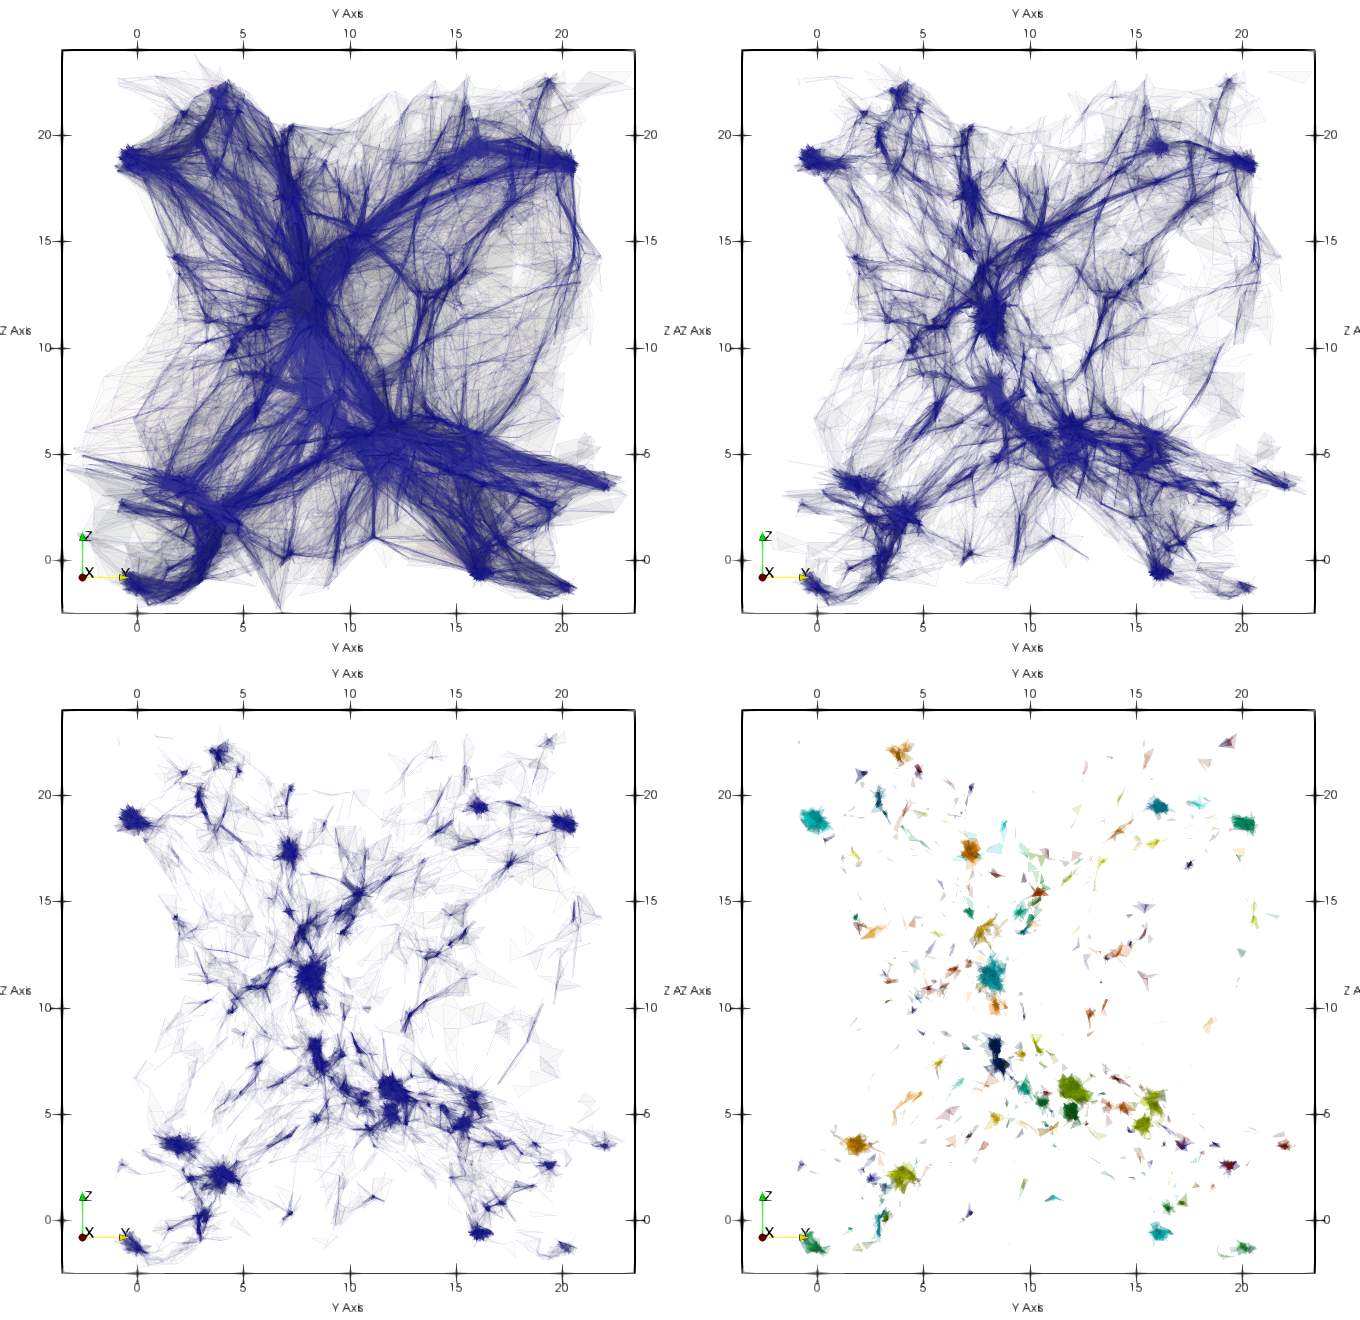
\includegraphics[height=15cm]{Chapter2/Plots/caustic_connectivity.png} 
\caption{Caustic surfaces in a small cosmological simulation of $L=20$ Mpc, $N_p = 32^3$. Caustics are filtered by longest side length $l_{max}$ of the triangle consitituting the caustic surface. Top left: all values of $l_{max}$ (all the caustic surfaces), top right: $ l_{max} \leq 1.8  h^{-1} Mpc$, bottom left: $ l_{max} \leq 1.25  h^{-1} Mpc$, bottom right: $ l_{max} \leq 1.0  h^{-1} Mpc$. Multiple colors in bottom right panel indicate isolated inner caustic surfaces, while the other three panels display connected outer cautic structures.}
\label{fig:caustic_lmax}
\end{figure*}

Despite the theoretical understanding mentioned above, delineating caustic surfaces at various levels of gravitational collapse has been proven to be difficult. Instead, a combination of geometric and topological methods may also enable us to trace the caustic formation. The DM particles on the caustics are on curved two dimensional surfaces, forming vertices of triangles that constitute the {\it tiles} of the surface. These triangles are of various shapes and size. Since the mean separation of particles is smaller than elsewhere in the cosmic web, the triangles are smaller on an average. Using the largest side of the triangle $l_{max}$ as a proxy for length scale of the triangle, one may perform morphological analyses on the type of caustic surfaces. One such study is shown in \autoref{fig:caustic_perc_lmax}. Percolation transitions (in an unstructured grid, as opposed to regular grid analyses for multistream or flip-flop fields) are used to differentiate the larger caustic surface (like the ones between voids and walls) and the smaller ones (like the concentric caustic shells around haloes). This transition in our small cosmological simulation of side length $L = 20 h^{-1} Mpc$ is seen at around $1.2 h^{-1} Mpc$. 


Using the heuristic parameter of $l_{max}$, we are able to isolate caustic surfaces around specific structures like the haloes. The \autoref{fig:caustic_lmax} shows all the caustic surfaces in the top left panel, and the inner caustics filtered using $l_{max}$ thresholds in the subsequent panels. Another interesting aspect of this filtering scheme is the ability to isolate the caustic surfaces around the haloes as seen in the bottom right panel of \autoref{fig:caustic_lmax}. 


Careful examination of the smaller caustic surfaces around the haloes may reveal concentric shells where the particles {\it turn back}. A spherical approximation of this, called the {\it splashback radius} \citep{More2015}. This has gained a considerable attention recently due to possible observational signatures of physical boundaries of dark matter haloes \citep{Chang2017}. Caustic finding scheme with appropriate filtering provides a general method to find these boundaries in N-body simulations exactly. Moreover, mapping caustic surfaces from Eulerian space to Lagrangian space displays concentric surfaces, providing a dynamical insight into the splashback radii of dark matter haloes. 



\section{Final remarks}

Understanding the complex dynamical processes that shape the dark matter web has been the primary focus of this thesis. By developing a wide variety of topological, geometrical and statistical diagnostic algorithms, we have demonstrated the potential of the Lagrangian sub-manifold in unveiling properties of the cosmic structures. Despite these modern advancements, the Zel'dovich approximation has to be recognized as the basis for a dynamical theory for the evolution of the dark matter web and its components. 

On the one hand, such a motivated theoretical framework may result in a systematic descriptor of the large scale dark matter structures in the Universe. On the other, perplexing complexities of halo substructures, caustic singularities and merger histories could be unmasked. This only demands extensive studies in the field of Physical cosmology.   


